\documentclass[a4paper,10pt]{article}

%%%%%%%%%%%%%%%%%%%%%%%%%%%%%%%%%%%%%%%%%
% packages
%%%%%%%%%%%%%%%%%%%%%%%%%%%%%%%%%%%%%%%%%
\usepackage{graphicx}
\usepackage{url}

\usepackage[utf8x]{inputenc}

\usepackage{graphicx}
\usepackage{amssymb}
\usepackage{amsmath}
\usepackage{lineno}
\usepackage{verbatim} 

\usepackage{array,float,epsf,psfrag,eurosym,theorem}
\usepackage{amsfonts}
\usepackage{bbm}
\usepackage{mathrsfs}

\usepackage{color}
\usepackage{srcltx}


\usepackage{geometry}
\usepackage{xspace}
\usepackage{bm}
\usepackage[figtopcap,tight,nooneline]{subfigure}
\usepackage{amssymb}

%%%%%%%%%%%%%%%%%%%%%%%%%%%%%%%%%%%%%%%%%
% definitions:
%%%%%%%%%%%%%%%%%%%%%%%%%%%%%%%%%%%%%%%%%
\newcommand{\reffig}[1]{Fig.~\ref{fig:#1}}
\newcommand{\reffigs}[2]{Figs.~\ref{fig:#1},~\ref{fig:#2}}
\newcommand{\refeq}[1]{Eq. (\ref{eq:#1})}
\newcommand{\refeqs}[2]{(\ref{eq:#1}),~(\ref{eq:#2})}
\newcommand{\reftab}[1]{Tab.~\ref{tab:#1}}
\newcommand{\reftabs}[2]{Tabs.~\ref{tab:#1},~\ref{tab:#2}}

\newcommand*{\QEDA}{\hfill\ensuremath{\blacksquare}}%
\newcommand*{\QEDB}{\hfill\ensuremath{\square}}%

%%%%%
\DeclareMathAlphabet{\mathpzc}{OT1}{pzc}{m}{it}

%\def\gz  #1{           \mbox{$\mathbf{#1}$}}
\def\gz  #1{           \mbox{\boldmath $\mit #1$}}
%\def\gzb #1{\overline {\mbox{\boldmath $\mit #1$}}}
\DeclareMathAlphabet{\bsf}{OT1}{cmss}{bx}{n}
\def\msf  #1{           \mbox{\!\!      $\sf #1$}}
\def\Grad #1 {{\rm Grad} #1}
\def\grad #1 {{\rm grad} #1}
\def\Div {\mbox{Div}}
\def\d {\,\mbox{d}}
\def\D {\,\mbox{D}}
\def\gzh #1{\widehat  {\mbox{\boldmath $\mit #1$}}}
\newcommand{\norm}[1]{\left\lvert #1 \right\rvert}
\newcommand\normDouble[1]{\left\lVert#1\right\rVert}
\newcommand{\normXY}[1]{\lvert #1 \rvert_{2d}}
\newcommand{\dbracket}[1]{\left[\!\!\left[ #1 \right]\!\!\right]}

\def\mcl  #1{               {\cal #1}}
\def\bcl  #1{\mbox{\boldmath$\cal #1$}}
\def\cc #1{\,{\mathbbm #1}}
\def\set #1{\mbox{I$\!$#1}}

%%%%%%%%%%%%%%%%%%%%%%%%%%%%%%%%%%%%%%%%%
% document:
%%%%%%%%%%%%%%%%%%%%%%%%%%%%%%%%%%%%%%%%%

\parindent0pt
\begin{document}


\section{Derivation of energy and forces}
The position vector for particle $\alpha$ in Euclidean space with origin $\bsf x = \gz 0$ is denoted by
\begin{align}
\bsf x^\alpha \in  \cc E^3.
\end{align}

In case of pair-potentials only, the total energy of the non-local quasi-continuum method is then defined as
\begin{align}
\begin{split}
\msf E &= \sum_{A \in \mcl C} n_A \msf E_A \\
           &= \sum_{A \in \mcl C} n_A \sum_{\alpha \in \mcl C_A} \msf E^\alpha \\
           &= \sum_{A \in \mcl C} n_A \sum_{\alpha \in \mcl C_A} \sum_{\beta \in \mcl N_\alpha} \frac{1}{2} \msf E^{\alpha \beta} (\msf r^{\alpha\beta}),
\end{split}
\end{align}
where $\mcl C$ is the set of all clusters, $\mcl C_A$ is the set of atoms attributed to the cluster $A$, $\mcl N_\alpha$ is the set of atoms which interact with atom $\alpha$,
$\msf E^{\alpha \beta}$ is the energy of the interaction between particles $\alpha$ and $\beta$, which depends on the distance between the two particles $\msf r^{\alpha\beta}$.

Unknown displacement field is given in the FE vector-valued functional space as
\begin{align}
\gz u (\gz x) = \sum_{i \in N_{dofs}} u_i \, \gz N_i (\gz x),
\end{align}
where $\gz N_i (\gz x)$ are vector-valued shape functions.


\begin{figure}[!ht]
   \centering
    \includegraphics[angle=90,width=0.98\textwidth]{mesh_clusters.001.png.ps}
    \caption{
        Treatment of hanging nodes for the $h$\,-adaptive QC method.
    }
    \label{fig:mesh_clusters}
\end{figure}

\begin{figure}[!ht]
    \centering
    \includegraphics[angle=90,width=0.98\textwidth]{mesh_clusters_mpi.001.png.ps}
    \caption{
        An example of partition of elements and DoFs among processors. Background colour for each DoF indicate which processor owns it.
    }
    \label{fig:mesh_mpi}
\end{figure}


Gradient of the total energy with respect to the unknown DoFs will require the following
\begin{align}
\frac{\partial \msf r^{\alpha \beta}}{\partial u_i} = \frac{\partial \msf r^{\alpha \beta}}{\partial \bsf r^{\alpha\beta}} \cdot \frac{\partial \bsf r^{\alpha\beta}}{\partial u_i} = \frac{\bsf r^{\alpha\beta}}{r^{\alpha\beta}} \cdot \frac{\partial \bsf r^{\alpha\beta}}{\partial u_i}
\end{align}
with
\begin{align}
\frac{\partial \gz r^{\alpha\beta}}{\partial u_i} = \frac{\partial\left[\bsf X^\alpha + \sum_l u_l \gz N_l(\bsf X^\alpha) - \bsf X^\beta - \sum_m u_m \gz N_m(\bsf X^\beta)\right]}{\partial u_i} = \gz N_i (\gz X^\alpha) - \gz N_i (\gz X^\beta)
\end{align}

Note the non-local nature of the assembly. The contribution to the gradient vector from each cell depends not only on the values of shape functions in this cell evaluated at $\bsf X^\alpha$, but also on values of the same shape function evaluated at points $\bsf X^\beta$ within its support on possibly neighbouring cells.

\begin{align}
\frac{\partial r^{\alpha\beta}}{\partial u_i} = \frac{\bsf r^{\alpha\beta}}{\msf r^{\alpha\beta}} \cdot \left[\gz N_i (\bsf X^\alpha) - \gz N_i (\gz X^\beta) \right]
\end{align}


Rewrite the total energy in the equivalent form
\begin{align}
\msf E &= \sum_{e \in \Omega} \sum_{\alpha \in \Omega_e} \sum_{\beta \in \mcl N_\alpha} \frac{1}{2} \left[n^\alpha + n^\beta\right] \msf E^{\alpha \beta} (\msf r^{\alpha\beta}),
\end{align}
where $\Omega$ is the set of all elements, $\Omega_e$ is the set of all atoms attributed to possibly different clusters within the element $e$ and $n^\alpha$ and $n^\beta$ are weights of atoms. Atoms not associated with any clusters have weights zero.


Some of the energies $\msf E^{\alpha\beta}$ will be evaluated twice. To circumvent this, we rewrite the energy as
\begin{align}
\msf E &= \sum_{e \in \Omega} \sum_{\alpha \in \Omega_e}
\left[
\sum_{\alpha < \beta \in \mcl N_\alpha^C} \left[n^\alpha + n^\beta\right] \msf E^{\alpha \beta} (\msf r^{\alpha\beta})
+
\sum_{\beta \in \mcl N_\alpha^G} \frac{1}{2} n^\alpha \msf E^{\alpha \beta} (\msf r^{\alpha\beta})
\right],
\end{align}
where $N_\alpha^C$ is a set of all atoms interacting with atom $\alpha$ and attributed to some cluster, whereas
$N_\alpha^G$ is a set of all ``ghost'' atoms, which are not attributed to any cluster.
$N_\alpha^G \cup N_\alpha^C = N_\alpha$ and $N_\alpha^G \cap N_\alpha^C =  0$.

\subsection{Hanging nodes}

The last issue to be discussed is hanging nodes constraints (see \reffig{mesh_clusters}). The position of hanging nodes are restricted to
be on center of faces. Thereby we can not guarantee with appropriate mesh-motion teqchniques (see Sec. ...) that there will be an atom
located at the hanging node. Consequently, no clusters are assigned to hanging nodes.

The presence of hanging nodes does not impose difficulties in calculation of energies as one only need to evaluate a displacement field on each atom /quadrature point to be able to evaluated interparticle distance in deformed configuration. However, certain care should be taken in calculation of gradients of energy. 

The constraints to produce a $C^0$ continuous displacement field can be written as
\begin{align}
u_j = \sum_{i \in \mcl N_{u}} c_{ji} u_i, \qquad   j \in \mcl N_{c} ,
\end{align}
where  $\mcl N_{u}$ is the set of all unconstrained dofs and $\mcl N_c$ is the set of constrained DoFs,
whose support point is a hanging node. The total set of DoFs is $\mcl N = \mcl N_c \cup \mcl N_u$ and $\mcl N_c \cap \mcl N_u = 0$.

For example the FE space illustrated on \reffig{mesh_clusters} will have the following constraint
\begin{align}
u_3 = \frac{1}{2} u_2 + \frac{1}{2} u_4,
\end{align}
among others. 
In local methods (such as small strain linear elasticity), incorporation of either of these constraints is trivial.


\begin{align}
\begin{split}
\forall u_i \in \mcl N_{u} \,: \quad 
\frac{\partial \msf E }{\partial u_i} 
= \sum_{j \in \mcl N} \frac{\partial \msf E }{\partial u_j} \frac{\partial u_j }{\partial u_i}  
= \frac{\partial \msf E }{\partial u_i} + \frac{\partial \msf E }{\partial u_k} c_{ki} .
\end{split}
\end{align}
Thus, similar to the local methods, one can perform local cell assembly without distinguishing between constrained and un-constrained DoFs.
The hanging nodes constrains are accounted only at the local contribution to the (gradient) vector is distributed to the global vector.

\subsection{Parallelization}


{\color{red}TODO}: discuss parallelization via MPI + TBB within locally owned cells. Also discuss why distributed triangulation can't be used and why each MPI core needs to know the whole geometry.

\subsection{A multi-field approach for ionic crystals}

Consider an atomistic system consisting of a single type of molecules.
Let $\bsf X_I$ be the location of molecule $I \in \mcl M$ in the initial 
configuration, where $\mcl M$ is the index set of all the molecules in the 
atomistic system. $\bsf X_I$ can the center of mass or center of geometry of 
the molecule $M$ or any other convenient convention to identify the location of 
the molecule $M$ in the initial configuration of the atomistic system. Let the 
atoms of a molecule of the ionic compound be enumerated or stamped as $i \in 
\mcl A$. The cardinality of the set $\mcl A$ is the atomicity of the molecule. 
For example, in the case of O$_2$ molecule the set $\mcl A := \left\lbrace 0,1 
\right\rbrace$. The initial position of the atom stamped $i$ of the molecule 
$I$ is
\begin{align}
 \bsf X_I ^i = \bsf X_I + \bsf R^i,
\end{align}
where $\bsf R^i$ is the shift vector of the atom stamped $i$ within the 
molecule $I$, i.e., the relative position vector from the location of the 
molecule $I$ to its atom stamped $i$.

To define the displacements of different atoms within a molecule we define
multiple displacement field variables in the finite element space. The 
displacement of atom stamped $i$ in the molecule $I$ can be 
evaluated as
\begin{align}
 \bsf x_I^i = \bsf X_I^i + \gz u^i(\bsf X_I),
 \label{eq:current_atom_pos}
\end{align}
where $\gz u^i( \gz x)$ is the unknown displacement field of atoms that are 
stamped as $a$,
\begin{align}
 \gz u^i (\gz x) = \sum_{d \, \in \, \mcl D} u^i_d \,\, \gz N_d (\gz x),
\end{align}
where $\gz N_d (\gz x)$ are vector-valued shape functions and $\mcl D$ is the 
set of all degrees of freedom enumerated at the mesh nodes, one set for each 
atom stamp.
Note that in \refeq{current_atom_pos} we evaluate the displacement fields at 
the location of the molecule. This allows us to place the mesh nodes at the 
location of molecules in the atomistic region and enumerate all the degrees of 
freedoms for atoms at the mesh nodes. It is as if we identify representative 
molecules (rep-molecules) in the entire atomistic system and place mesh nodes 
at the location of rep-molecules.

The total energy would then read as,
\begin{align}
 E^{tot} = &\sum_{I \, \in \, \mcl C} w^{}_I \,\,
            \left[
		  E^{}_{II} +
		  \sum_{\mcl M \, \ni \, J < I} 
                  E^{}_{IJ} 
            \right]
\end{align}
where $\mcl C$ is the set of all sampling molecules, $w^{}_I$ is the cluster 
weight of sampling molecule $I$ and $E^{}_{IJ}$ is the contribution of energy 
due to the two interacting molecules $I$ and $J$ given as,
\begin{equation}
 E^{}_{IJ} =  \begin{cases}                   \,\,
               \sum\limits_{i \, \in \, I}    \,\,
               \sum\limits_{j \, \in \, J}    \,
		\phi^{}_{ij}(r^{jk}),
		& \text{if } \,  I \neq J \\[1em] \,\,

               \sum\limits_{i \, \in \, I}    \,\,
               \sum\limits_{J \, \ni \, j \, < \, i} \,
               \phi^{}_{ij}(r^{jk}), 
               & \text{otherwise}.
              \end{cases}
\label{eq:inter_and_intra}
\end{equation}
where $\phi^{}_{ij}(r^{jk})$ describes the interaction potential between two 
atoms with atom stamps $i$ and $j$ as a function of their separation distance 
$r^{jk} = \norm{\bsf r^{jk}} = \norm{ \bsf x^{i}_{I} - \bsf x^{j}_{J} }$. 
The gradient of the total energy with respect to the degree of freedom $d \in 
\mcl D$ of the atoms with atom stamp $k \in \mcl A$ is
\begin{align}
 g^k_d = &\sum_{I \, \in \, \mcl C}  \, w^{}_I \,\, 
	  \left[
		\frac{\partial E^{}_{II}}{\partial u^k_d}
		+
		\sum_{\mcl M \, \ni \, J < I}  \,
		\frac{\partial E^{}_{IJ}}{\partial u^k_d}
	   \right].
\end{align}
Using \refeq{inter_and_intra},
\begin{align}
 g^k_d = \sum_{I \, \in \, \mcl C}  \, w^{}_I
          \Bigg[
            \,\,\,\,\,\,\,\,\,\,\,\,\,\,\,\,\,\,\,\,\,\,\,
	    \sum_{i \, \in \, I}                          \,\,
	    \sum_{I \, \ni \, j \, < \, i}                \,
             &\frac{\partial \phi^{}_{ij}(r^{jk})}{\partial r} \, 
               \frac{\partial r^{jk}}{\partial \bsf r^{jk}} \cdot
               \frac{\partial \bsf r^{jk}}{\partial u^k_d}     \\
	    +
	    \sum_{\mcl M \, \ni \, J < I}  \,\,
            \sum_{i \, \in \, I}           \,\,
	    \sum_{j \, \in \, J}           \,
               &\frac{\partial \phi^{}_{ij}(r^{jk})}{\partial r^{jk}} \, 
                 \frac{\partial r^{jk}}{\partial \bsf r^{jk}} \cdot
                 \frac{\partial \bsf r^{jk}}{\partial u^k_d}
           \Bigg],
\end{align}
and on using \refeq{current_atom_pos},
\begin{align}
 g^k_d = \sum_{I \, \in \, \mcl C}  \, w^{}_I
	  \Bigg[
		\,\,\,\,\,\,\,\,\,\,\,\,\,\,\,\,\,\,\,\,\,\,\,
		\sum_{i \, \in \, I}       \,\,\,
		\sum_{I \, \ni \, j \, < \, i}       \,
		  &{\phi}^\prime_{ij} (r^{jk})\, \, 
		    \frac {\bsf r^{jk}}{r^{jk}}
		    \cdot
		    \bigg[
		      \delta_{ik} \,\, \gz N_d( \bsf X_{I})  
		      - 
		      \delta_{jk} \,\, \gz N_d( \bsf X_{I})
		    \bigg] \\
	      +
	      \sum_{\mcl M \, \ni \, J < I}  \,
	      \sum_{i \, \in \, I}       \,\,\,
	      \sum_{j \, \in \, J}       \,
		&{\phi}^\prime_{ij} (r^{jk})\, \, 
		  \frac {\bsf r^{jk}}{r^{jk}}
		  \cdot
		  \bigg[
		    \delta_{ik} \,\, \gz N_d( \bsf X_{I})  
		    - 
		    \delta_{jk} \,\, \gz N_d( \bsf X_{J})
		  \bigg]
	 \Bigg],
\end{align}
factoring out the shape function evaluations at molecules' locations we have
\begin{align}
 g^k_d = \sum_{I \, \in \, \mcl C}  \, w^{}_I
	  \Bigg[
		\,\,\,\,\,\,\,\,\,\,\,\,
		\,\,\,\,\,\,\,\,\,\,\,\,
		\,\,\,\,\,\,\,\,\,\,\,\,
		\,\,\,\,\,\,\,\,\,\,\,\,
		\gz N_d( \bsf X_{I})
		&\cdot
		  \sum_{i \, \in \, I}            \,\,\,
		  \sum_{I \, \ni \, j \, < \, i} \,
		  \frac {\bsf r^{jk}}{r^{jk}}               \,
		    {\phi}^\prime_{ij} (r^{jk})        \,
		      \Big(
			\delta_{ik} 
			- 
			\delta_{jk}
		      \Big)
		\\
	      + \,
		\sum_{\mcl M \, \ni \, J < I}  \,
		\Bigg\{
		  \,\,\,\,\,\,\,
		  \gz N_d( \bsf X_{I})
		  &\cdot
		    \sum_{i \, \in \, I}    \,\,\,\,\,
		    \sum_{j \, \in \, J}   \,
		    \frac {\bsf r^{jk}}{r^{jk}}       \,
		      {\phi}^\prime_{ij}(r^{jk}) \,
		      \delta_{ik}           \,
		    \\
		  -
		  \gz N_d( \bsf X_{J})
		  &\cdot
		    \sum_{i \, \in \, I}    \,\,\,\,\,
		    \sum_{j \, \in \, J}   \,
		    \frac{\bsf r^{jk}}{r^{jk}}
		      {\phi}^\prime_{ij}(r^{jk}) \,
		      \delta_{jk}           \,
		\,\,\,
		\Bigg\}
		\,\,\,\,\,\,\,\,\,\,\,\,
		\,\,\,\,\,\,\,\,\,\,\,\,
		\,\,\,\,\,\,\,\,\,\,\,\,
	 \Bigg],
\end{align}
where $r^{jk} = \norm{\bsf r^{jk}} = \norm{ \bsf x^{i}_{I} - \bsf x^{j}_{J} }$.
\end{document}
